% !TeX program = pdflatex
% !TeX encoding = UTF-8
%=======================================================================
%  GRIS-NOT-001  ·  Plantilla de notas rápidas para la memoria
%  Proyecto 00503 - Generator inspection robotic system · Mecanalisis
%  Identidad: GRIS-IDENTIDAD-001 v1.4
%-----------------------------------------------------------------------
%  CÓMO USARLA (en 3 pasos)
%
%   1. Copiá este archivo con el código de la nota:
%         memoria/notas/02489-00-MC007.tex
%      El número (###) es correlativo: mirá la última nota y sumá uno.
%
%   2. Completá los cuatro datos del bloque «DATOS DE LA NOTA».
%
%   3. Escribí:
%        · Resultados (obligatorio, siempre primero): lo que se sabe
%          ahora que antes no se sabía. Frases cortas, con números.
%        · El resto es libre. Usá los títulos que te sirvan, o ninguno.
%
%   Compilar:  pdflatex 02489-00-MC007.tex
%   En Overleaf: subí el .tex y logo-gris.pdf.
%
%  LOGO: se usa «logo-gris.pdf» (GRIS-LOGO-003, reducido) de esta carpeta
%  o de ../plantilla/. Si falta, se escribe «GRIS» como marcador.
%=======================================================================
\documentclass[11pt,a4paper]{article}

%=======================================================================
%  DATOS DE LA NOTA  ← lo único que hay que tocar arriba
%=======================================================================
\newcommand{\codigo}{02489-00-MC002}          % 02489-00-MC###
\newcommand{\titulo}{Grado del imán con entrehierro de 1,5~mm}
\newcommand{\autor}{Matías Gaviño}
\newcommand{\fecha}{24/09/2026}                    % o p. ej. {24/09/2026}

%=======================================================================
%  ESTILO  (no hace falta tocar nada de aquí hasta \begin{document})
%=======================================================================
\usepackage[T1]{fontenc}
\usepackage[utf8]{inputenc}
\usepackage[spanish,es-noshorthands,es-tabla]{babel}
\usepackage{lmodern}
\usepackage[a4paper,top=3.0cm,bottom=2.4cm,left=2.4cm,right=2.4cm,
            headheight=20pt,headsep=1.2cm,footskip=1.1cm]{geometry}
\usepackage{microtype}
\usepackage{xcolor}
\usepackage{graphicx}
\usepackage{booktabs}
\usepackage{array}
\usepackage{enumitem}
\usepackage{titlesec}
\usepackage{fancyhdr}
\usepackage{caption}
\usepackage{amsmath}
\usepackage{float}
\usepackage[hidelinks]{hyperref}

% --- colores -----------------------------------------------------------
\definecolor{gris-naranja}{HTML}{FF7A00}   % naranja institucional
\definecolor{tinta}{HTML}{1E2328}
\definecolor{gris-medio}{HTML}{6B7280}
\definecolor{gris-linea}{HTML}{DADDE1}
\color{tinta}

\hypersetup{pdftitle={\codigo\ -- \titulo}, pdfauthor={\autor},
            colorlinks=true, linkcolor=tinta, urlcolor=tinta}

% --- logo ---------------------------------------------------------------
\graphicspath{{./}{../plantilla/}{plantilla/}}
\newcommand{\logogris}{%
  \IfFileExists{logo-gris.pdf}
    {
\includegraphics[height=16pt]{logo-gris.pdf}}
    {\IfFileExists{../plantilla/logo-gris.pdf}
      {
\includegraphics[height=16pt]{../plantilla/logo-gris.pdf}}
      {{\fontsize{18}{18}\selectfont\bfseries\sffamily\color{gris-naranja}GRIS}}}}

% --- tipografía del cliente (código documental) --------------------------
% Geogrotesque no es libre; se usa Roboto Condensed Bold, que viene con
% TeX Live y Overleaf y tiene el mismo aire que el logo.
\newcommand{\fuentecliente}{\fontfamily{Roboto-TLF}\fontseries{bc}\selectfont}

% --- encabezado y pie ---------------------------------------------------
\pagestyle{fancy}
\fancyhf{}
\renewcommand{\headrulewidth}{0.4pt}
\renewcommand{\headrule}{\vspace{3pt}{\color{gris-linea}\hrule height \headrulewidth}}
\fancyhead[L]{\logogris}
\fancyhead[R]{{\fuentecliente\fontsize{12}{12}\selectfont\color{gris-medio}\codigo}}
\fancyfoot[R]{\footnotesize\color{gris-medio}\thepage}

% --- títulos numerados ----------------------------------------------------
\setcounter{secnumdepth}{2}
\titleformat{\section}{\large\bfseries}{\thesection}{0.8em}{}
\titleformat{\subsection}{\normalsize\bfseries}{\thesubsection}{0.8em}{}
\titlespacing*{\section}{0pt}{16pt}{5pt}
\titlespacing*{\subsection}{0pt}{11pt}{3pt}

% --- texto ------------------------------------------------------------------
\setlength{\parindent}{0pt}
\setlength{\parskip}{6pt}
\linespread{1.05}
\setlist{topsep=2pt, itemsep=2pt, parsep=0pt, leftmargin=1.2em}
\setlist[itemize]{label={\raisebox{0.15ex}{\small$\bullet$}}}
\captionsetup{font={small,color=gris-medio}, labelfont=bf, skip=5pt}
\renewcommand{\arraystretch}{1.25}

% --- cabecera de la nota ------------------------------------------------------
\newcommand{\cabecera}{%
  \thispagestyle{fancy}%
  {\fontsize{20}{24}\selectfont\bfseries\titulo\par}%
  \vspace{5pt}%
  {\small\color{gris-medio}\fecha\quad·\quad\autor\par}%
  \vspace{6pt}}

% --- ayudas opcionales --------------------------------------------------------
% \figura{archivo}{ancho}{pie}
\newcommand{\figura}[3]{%
  \begin{figure}[htbp]\centering
    \includegraphics[width=#2\linewidth]{#1}\caption{#3}
  \end{figure}}

%=======================================================================
\begin{document}
\cabecera

%-----------------------------------------------------------------------
%  RESULTADOS  (siempre primero, lo único obligatorio)
%-----------------------------------------------------------------------
\section{Resultados}
El montaje impone un entrehierro mínimo de 1,5~mm entre el conjunto de dos imanes D20$\times$4
avellanados y el acero. Se evaluó cambiar los imanes actuales (se comportan como \textbf{N35},
informe 02489-00-ZIT200) por N42 o N52, cambiando solo el imán o agregando un separador que
mantiene la fuerza a 1,5~mm en el valor actual.

\begin{table}[H]\centering\small
\begin{tabular}{l c c c c c}
\toprule
Variante & Separador & $F(1{,}5\text{ mm})$ & $\Delta F_{\text{máx}}$ & $x$ a 2~N & Ganancia\\
         & [mm]      & [N]                 & [\%]                  & [mm]      & [mm]\\
\midrule
N35 actual (referencia) & --   & 25,6           & --      & 9,85  & --\\
N42 sin separador       & --   & $\approx$30,6  & +19     & 10,65 & +0,80\\
N42 + separador         & 0,37 & 25,6           & 0       & 10,28 & +0,43\\
N52 sin separador       & --   & $\approx$38    & +48     & 11,69 & +1,84\\
N52 + separador         & 0,88 & 25,6           & 0       & 10,81 & +0,96\\
\bottomrule
\end{tabular}
\end{table}

\begin{itemize}
  \item \textbf{Fuerza máxima utilizable actual: 25,6~N} a 1,5~mm, poco más de un tercio de los
        68,7~N medidos en contacto. El tramo por debajo de 1,5~mm no es accesible.
  \item \textbf{Cambiar solo el imán} sube la fuerza máxima a $\approx$30,6~N (N42, +19\,\%) o
        $\approx$38~N (N52, +48\,\%), y lleva el alcance a 2~N de 9,85 a 10,65~mm (N42) o 11,69~mm (N52).
  \item \textbf{Manteniendo la fuerza máxima en 25,6~N} hace falta un separador de 0,37~mm (N42) o
        0,88~mm (N52), y el alcance a 2~N mejora solo \textbf{0,43~mm} y \textbf{0,96~mm}.
  \item \textbf{El grado del imán mueve la cola de la curva menos de 2~mm} en el mejor caso. No
        justifica el cambio si el objetivo es alcance; sí, si falta fuerza cerca y el sistema tolera
        el aumento.
  \item \textbf{Siguiente paso:} para ganar alcance, evaluar variantes geométricas (volumen y altura
        del imán, retorno de flujo por la cara opuesta, espesor del blanco) con el modelo FEMM ya validado.
\end{itemize}

\begin{figure}[H]\centering
  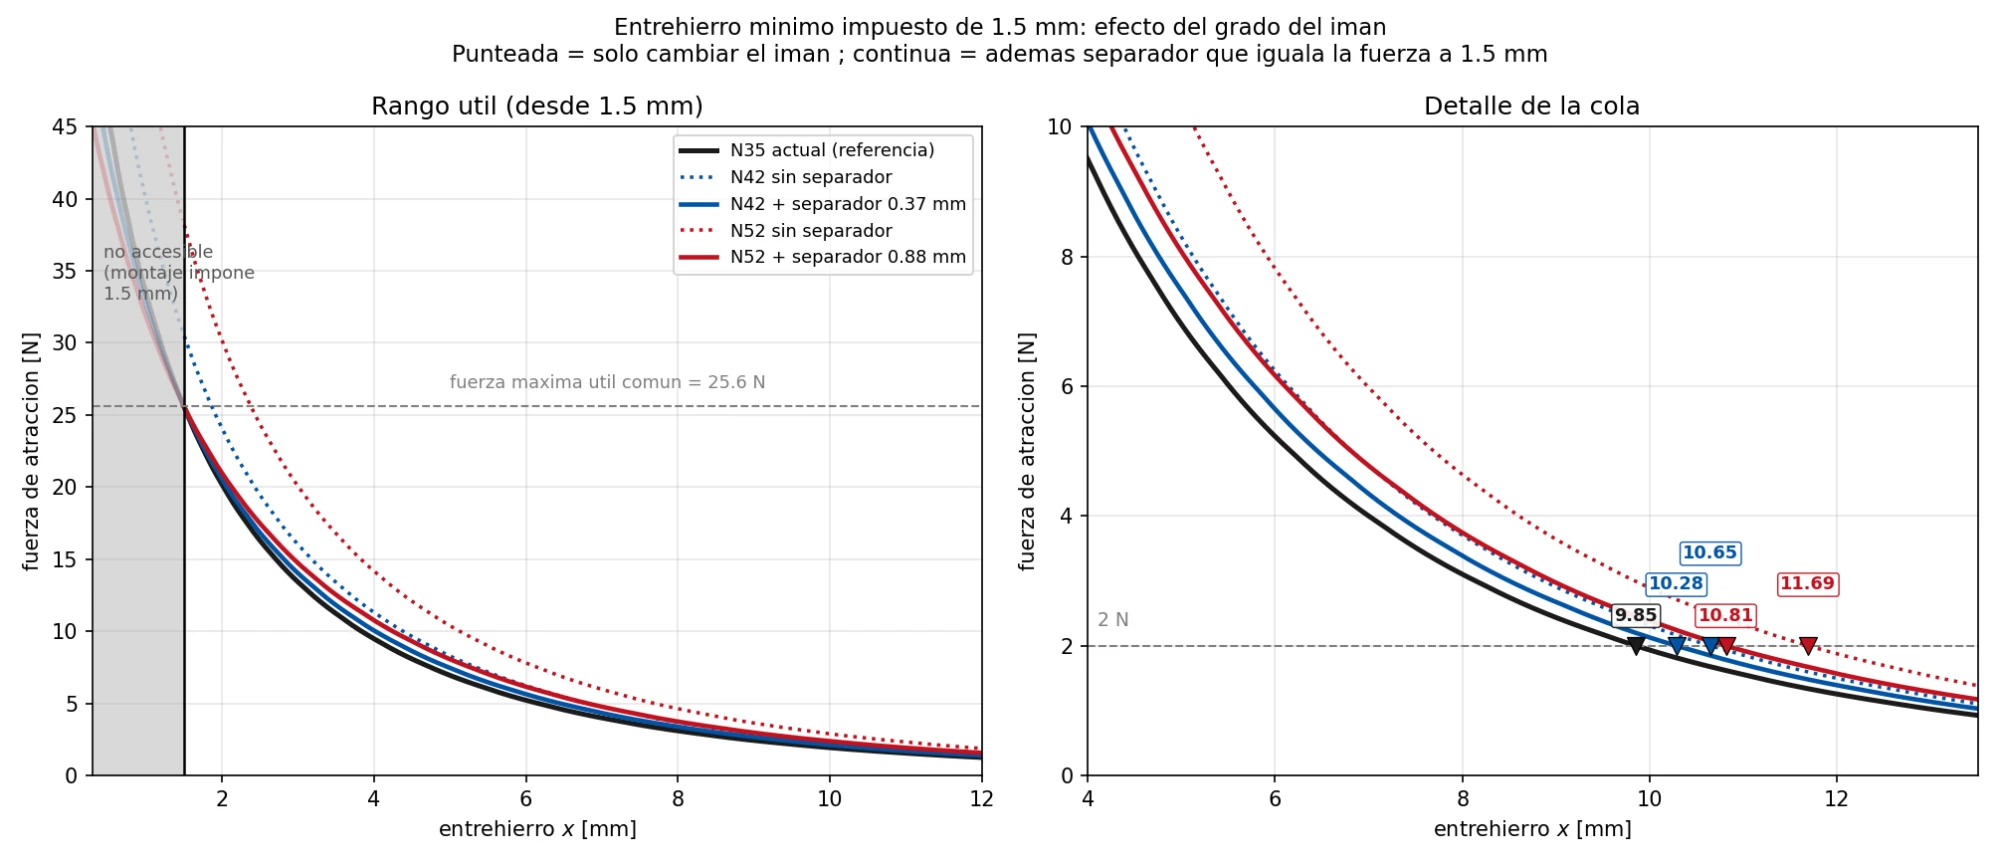
\includegraphics[width=\linewidth]{02489-00-MC002/figuras/fig_grado_entrehierro.png}
  \caption{Fuerza de atracción con entrehierro mínimo de 1,5~mm. Negro: conjunto actual. Punteadas:
  solo cambiar el imán. Continuas: imán más separador que iguala la fuerza a 1,5~mm. Los triángulos
  marcan el entrehierro al que cada curva cae a 2~N.}
  \label{fig:grado}
\end{figure}

%-----------------------------------------------------------------------
\section{Datos y supuestos}

\begin{table}[H]\centering\small
\begin{tabular}{l l l}
\toprule
Dato & Valor & Origen\\\midrule
Entrehierro mínimo & 1,5~mm & montaje\\
Curva de referencia & FEMM ajustada, $B_r$ efectivo 1,051~T & 02489-00-ZIT200, tabla 1\\
$B_r$ nominal N35 / N42 / N52 & 1,19 / 1,30 / 1,45~T & catálogo\\
Umbral de alcance & 2~N & criterio de comparación\\
Separador & No magnético, espesor uniforme & \textbf{supuesto}\\
\bottomrule
\end{tabular}
\end{table}

Mientras el acero no sature, la fuerza escala con el cuadrado de la remanencia (02489-00-ZIT200,
ec.~2). Cada grado se obtiene escalando la curva actual; el separador de espesor $s$ suma
entrehierro a toda la curva:
\begin{equation}
F_g(x)=\left(\frac{B_{r,g}}{B_{r,\text{N35}}}\right)^{2} F_{\text{N35}}(x+s).
\end{equation}
Los factores de fuerza son 1,19 (N42) y 1,48 (N52). El separador se elige para que
$F_g(1{,}5\text{ mm})=25{,}6$~N. El cálculo está en \texttt{02489-00-MC002/calculo.py}
y sus resultados en \texttt{resultados.json}; los alcances a 2~N salen de las curvas FEMM de la
figura~\ref{fig:grado}.

%-----------------------------------------------------------------------
\section{Por qué el alcance crece tan poco}

\paragraph{La fuerza crece mucho más que el alcance.}
En la cola, la fuerza cae a la mitad cada 2,5 a 3~mm. Un factor constante en la fuerza se
traduce en un corrimiento acotado del entrehierro: del orden de 0,4~mm por cada 10\,\% de fuerza
adicional. Por eso el N52, con +48\,\% de fuerza, gana solo 1,84~mm.

\paragraph{El separador consume parte de la ganancia.}
El separador corre toda la curva en $s$: el alcance con separador es el alcance sin separador
menos $s$ (10,65 $-$ 0,37 = 10,28~mm; 11,69 $-$ 0,88 = 10,81~mm). Como la curva decae más rápido
cerca del imán que en la cola, un separador delgado basta para absorber el aumento de fuerza a
1,5~mm, y en la cola sobrevive aproximadamente la mitad de la ganancia.

%-----------------------------------------------------------------------
\section{Limitaciones}
\begin{itemize}
  \item \textbf{Grado real de los imanes actuales.} Se comportan como N35, pero según
        02489-00-ZIT200 (sec.~6) el grado real puede ser N35 o algo superior. Si fuera mayor, la
        ganancia por cambiar de imán sería menor que la informada.
  \item \textbf{Pérdidas del ensayo trasladadas.} Escalar la curva medida supone que la pintura, el
        espesor finito del blanco y la desalineación afectan a todos los grados por igual. Vale
        mientras el acero no sature, condición que el N52 a 1,5~mm exige más.
  \item \textbf{Remanencias de catálogo.} Dentro de un grado, $B_r$ varía algunos puntos porcentuales
        entre fabricantes: el doble en fuerza.
  \item \textbf{Cola de la curva.} La referencia hereda la tendencia de los residuos de
        02489-00-ZIT200 (sec.~5.3): en la cola el modelo supera a la medición hasta un 20\,\%. Los
        alcances absolutos pueden estar sobreestimados en algunas décimas de milímetro; las
        diferencias entre grados, mucho menos.
\end{itemize}

\end{document}
